\documentclass{article}
\usepackage[utf8]{luainputenc}
\usepackage[T1]{fontenc}
\usepackage[a4paper,margin=0.75in, bottom=1in]{geometry}
\usepackage{listings}
\usepackage{courier}
\usepackage{amsmath}
\usepackage{amssymb}
\usepackage{enumerate}
\usepackage{graphicx}
\usepackage{hyperref}

\begin{document}
	
	\hrulefill
	\begin{center}
		\bfseries % Fettdruck einschalten
		\sffamily % Serifenlose Schrift
		\begin{huge}
			GTI: Grundlagen der Theoretischen Informatik
		\end{huge}\\
		\begin{Large}
			Sommersemester 2017, 4. Übungsblatt
		\end{Large}\\
		\begin{small}
			Valentin Wolf, Luis Herrmann; Tutor: Kristin Knorr; Mo 12:00-14:00
		\end{small}
		
		\vspace{-10pt}
	\end{center}
	\hrulefill
	
\section*{Aufgabe 1 - \textit{Mealy-Automaten}}
Wir konstruieren einen Automaten $(Q, \Sigma, \Sigma', \delta: Q\times \Sigma \to Q \times \Sigma', q_0)$ über $\Sigma = \Sigma' = \{0,1\}$, der folgendes leistet: Die Bits and jeder 2. und an jeder 5. Stelle werden unverändert gelassen. Alle anderen Bits werden gekippt.\\

Es ist naheliegend, dass man für die Konstruktion des Automaten mindestens $kgV(2,5) = 10$ Zustände braucht, also wählen wir Zustände $Q := \{q_0,q_1,...,q_9\}$. Die Überführungsfunktion ist dann einfach zu definieren:
\begin{equation}
	\delta(q_n,a) = \begin{cases}
	(q_{n+1}\text{ mod } 10,a), &n+1 \text{ mod } 2 = 0 \lor n+1 \text{ mod } 5 = 0\\
	(q_{n+1}\text{ mod } 10,1-a), &\text{sonst}
	\end{cases}
\end{equation}

Grafisch sieht das dann wie folgt aus:

\begin{minipage}{\textwidth}
	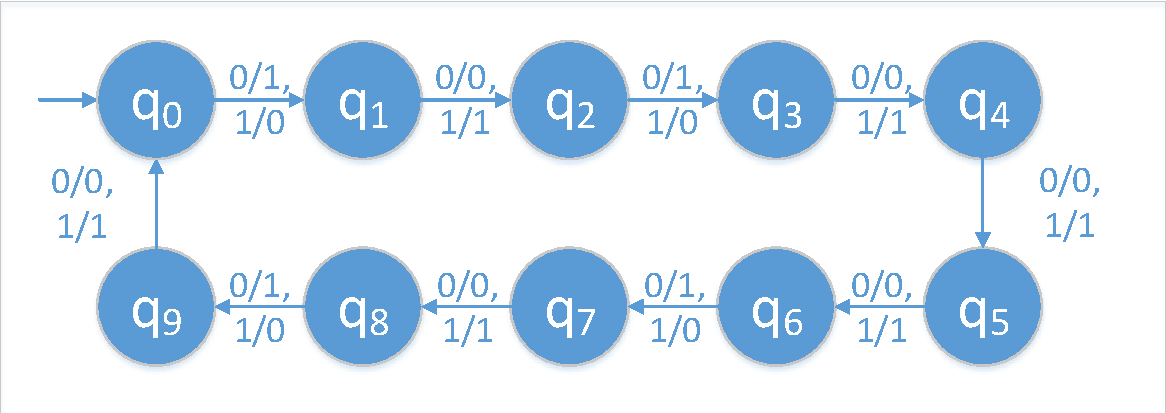
\includegraphics[width=\textwidth,page=1,trim={2 2 2 4},clip]{automaten.pdf}
\end{minipage}

\section*{Aufgabe 2 - \textit{Nichtregulär I}}

Wir wollen per Widerspruchsbeweis zeigen, dass die Sprache $L= \{0^p | p \text{ prim }\}$ nicht regulär ist. Dazu wenden wir das Pumping-Lemma an. Sei $A$ ein Automat, der $L$ akzeptiert, mit $n$ Zuständen. Sei $p \ge n$ eine beliebige Primzahl. Dann ist $0^p$ ein Wort aus der Sprache und gemäß Pumping-Lemma existiert eine Zerlegung $0^p = uvw$ mit $|uv| \le n $, $|v| \ge 1$, sodass $\forall i \ge 1 : uv^i w \in L$, also wieder eine unäre Kodierung einer Primzahl.\\


Offenbar besteht das Wort nur aus Nullen, also $uvw = 0^{|u|} 0^{|v|} 0^{|w|}$. Dann gilt aber:
\begin{equation}
	uv^i w = 0^{|u|} 0^{|v|} 0^{|w|} = 0^{|u|} (0^{|v|})^i 0^{|w|} = 0^{|u| + i|v| + |w|}
\end{equation}

Offenbar ist $i = |u| + |w|$ eine natürliche Zahl mit $i \ge 1$, da $|w| \ge 1$ und für dieses $i$ gilt:
\begin{equation}
	uv^{|u| + |w|} w = 0^{|u| + |v|(|u| + |w|) + |w|} = 0^{(|u| + |w|)(|v|+1)}
\end{equation}

Aber $(|u| + |w|)(|v|+1)$ ist keine Primzahl im Widerspruch zum Pumping-Lemma, also kann es keinen Automaten $A$ geben, der $L$ akzeptiert und wir haben damit gezeigt, dass die Sprache nicht regulär ist.

\section*{Aufgabe 3 - \textit{Nichtregulär II}}
\begin{enumerate}[a)]
	\item Wir zeigen, dass die Sprache $L_k := \{0^k 1^{n-k} 0^n | n \ge k \}$ für jedes feste $k$ nicht regulär ist. Sei $A_L$ ein Automat, der die Sprache akzeptiert mit $n$ Zuständen. Wir wählen ein $z = 0^k 1^{n-k} 0^{n}$ mit $z \in L$ mit $|z| = 2n$. Sei $uvw = z$ eine Zerlegung von $z$ mit $|uv| \le n$ und $|v| \ge 1$.
	
	\begin{enumerate}
		\item[1.Fall] $|uv| \le k \le n$. Dann ist $uv = 0^{|uv|}$ und $v = 0^{|v|}$. Also gilt:
		
		\begin{align}
			uv^iw &= 0^{|u|} (0^{|v|})^i 0^{k - |uv|} 1^{n-k} 0^n\\
			&= 0^{|u|+|v|i + k -|uv|} 1^{n-k} 0^n\\
			&= 0^{k + |v|(i-1)}1^{n-k} 0^n
		\end{align}
		
		Da $|v| \ge 1$ ist $k + |v|(i-1) > k $ für alle $i\ge 2$ und somit liegt das Wort nicht in $L$.
		
		\item[2.Fall] $k < |uv| \le n$. Dann ist $uv = 0^k 1^{|uv| - k}$.
		\begin{enumerate}
			\item[2.1] $|u| \ge k$, also $v = 1^{|uv|-|u|} = 1^{|v|}$.
			
			\begin{align}
				uv^i w &= 0^k 1^{|u|-k} (1^{|v|})^i 1^{n-|uv|}0^n\\
				&= 0^k 1^{|u| - k + |v|i + n -|uv|} 0^n\\
				&= 0^k 1^{n-k + |v|(i-1)} 0^n
			\end{align}
			
		Da $|v| \ge 1$ ist $n - k + |v|(i-1) > n-k$ für alle $i\ge 2$ und somit liegt das Wort nicht in $L$.\\
			
			\item[2.2] $|u| < k$. Dann ist $u = 0^{|u|}$ und $v = 0^{k-|u|}1^{|uv|-k}$.
			
			\begin{align}
				uv^i w &= 0^{|u|} (0^{k-|u|} 1^{|uv|-k})î 1^{n-|uv|} 0^n\\
				&= 0^{|u|+(k-|u|)i} 1^{n-k + (|uv|-k)(i-1)} 0^n
			\end{align}
			
			Da nach Voraussetzung $|uv| > k$ ist $n-k + (|uv|-k)(i-1) > n-k$ für $i \ge 2$ und somit liegt das Wort nicht in $L$.
		\end{enumerate}
	\end{enumerate}

	Damit haben wir für alle möglichen Zerlegungen des Wortes gezeigt, dass ein $i$ existiert, sodass $uv^iw \not\in L$ im Widerspruch zum Pumping-Lemma. Also kann $L_k$ nicht reguläre Sprache sein.
	
	\item Wir zeigen die Nichtregularität der Sprache $ADD := \{x = y + z \in \Sigma^* | x,y,z \text{ sind Binärzahlen mit } x = y + z \}$, wobei $\Sigma = \{0,1,+,=\}$. Sei $n$ die Zustandszahl eines potenziellen Automaten $A_{ADD}$. Wähle ein Wort $\omega \in L$, $|w| \ge n$, welches folgende Form hat:
	\begin{equation}
		"x_1x_2...x_{n+1} = y_1 ... y_n + z_1 ... z_n"
	\end{equation}
	
	Dabei setzen wir voraus, dass $x_1, y_1, z_1 = 1$. Betrachten wir eine beliebige Zerlegung $\omega = uvw$ mit $|uv| \le n$ und $|v| \ge 1$, dann ist also $uv = "x_1x_2...x_{|uv|}$ und $v = x_{|uv| - |v| + 1} ... x_{|uv|}$. Für eine beliebige Zerlegung gilt dann also:
	\begin{equation}
		uv^i w = "x_1x_2 ... (x_{|uv| - |v| +1 } ... x_{|uv|})^i ... x_{n+1} = y_1...y_n +  z_1 ... z_n"
	\end{equation}
	
	Offenbar gilt aber $x_1x_2 ... (x_{|uv| - |v| +1 } ... x_{|uv|})^i ... x_{n+1} > x_1x_2... x_{n+1} = y_1...y_n z_1 ... z_n$ für alle $i > 1 $ und somit ist $uv^iw \not \in ADD$ im Widerspruch zum Pumping-Lemma.
	
	\item $L := \{w\bar{w} | w \in \Sigma^* \}$ über $\Sigma = \{0,1\}$ ist nicht-reguläre Sprache. Nehmen wir an, es gäbe einen dfa $A$ mit $n$ Zuständen, der $L$ akzeptiert. Sei $z \in L$ mit $|z| = 2n \ge n$, genauer $z = 0^n 1^n$. Sei $uvw = z$ eine Zerlegung von $z$ mit $|uv| \le n$ und $|v| \ge 1$. Dann gilt aber:
	\begin{equation}
		uv^i w = 0^{|u|} (0^{|v|})^i 1^n = 0^{|u| + |v|i} 1^n = 0^{n + |v|(i-1)} 1^n
	\end{equation}
	
	Für alle geraden $i-1$ mit $i > 2$ liegt das Wort nicht in der Sprache, denn dann wäre für $\alpha := \frac{|v|(i-1)}{2}$:
	\begin{equation}
		0^{\alpha}1^n = \overline{(0^n 0^\alpha)} = 1^n 1^{\alpha}
	\end{equation}
	
	Damit haben wir einen Widerspruch zum Pumping-Lemma konstruiert und die Sprache kann somit nicht regulär sein.
	
\end{enumerate}


\end{document}